\documentclass[article]{jss}

%%%%%%%%%%%%%%%%%%%%%%%%%%%%%%
%% declarations for jss.cls %%%%%%%%%%%%%%%%%%%%%%%%%%%%%%%%%%%%%%%%%%
%%%%%%%%%%%%%%%%%%%%%%%%%%%%%%

%% almost as usual
\author{Joseph Kelly\\Harvard University \And 
             Carl Morris\\ Harvard University\And
             Hyungsuk Tak\\Harvard University }
\title{\pkg{Rgbp}: Bayesian Hierarchical Modeling and Frequentist Method Check}

%% for pretty printing and a nice hypersummary also set:
\Plainauthor{Joseph Kelly, Carl Morris, Hyung Suk Tak} %% comma-separated
\Plaintitle{Rgbp: Bayesian Hierarchical Modeling and Frequentist Method Check} %% without formatting

%% an abstract and keywords
\Abstract{Bayesian-frequentist reconciliation via Bayesian hierarchical modeling for Gaussian, Binomial, and Poisson data and frequentist method check for good coverage probability.}
\Keywords{hierarchical model, multilevel model, random effects mixed model, method check, coverage probability, normal, binomial, poisson, shrinkage, \proglang{R}}
\Plainkeywords{keywords, comma-separated, not capitalized, r} %% without formatting
%% at least one keyword must be supplied

%% publication information
%% NOTE: Typically, this can be left commented and will be filled out by the technical editor
%% \Volume{50}
%% \Issue{9}
%% \Month{June}
%% \Year{2012}
%% \Submitdate{2012-06-04}
%% \Acceptdate{2012-06-04}

%% The address of (at least) one author should be given
%% in the following format:
\Address{
  Joseph Kelly\\
  Department of Statistics\\
  Harvard University\\
  1 Oxford Street, Cambridge, MA\\
  E-mail: \email{kelly2@fas.harvard.edu}\\
  URL: \url{http://www.people.fas.harvard.edu/~kelly2/}\\

  Carl Morris\\
  Department of Statistics\\
  Harvard University\\
  1 Oxford Street, Cambridge, MA\\
  E-mail: \email{morris@fas.harvard.edu}\\

  Hyungsuk Tak\\
  Department of Statistics\\
  Harvard University\\
  1 Oxford Street, Cambridge, MA\\
  E-mail: \email{hyungsuk.tak@gmail.com}\\

}

%% It is also possible to add a telephone and fax number
%% before the e-mail in the following format:
%% Telephone: +43/512/507-7103
%% Fax: +43/512/507-2851

%% for those who use Sweave please include the following line (with % symbols):
%% need no \usepackage{Sweave.sty}

%% end of declarations %%%%%%%%%%%%%%%%%%%%%%%%%%%%%%%%%%%%%%%%%%%%%%%

\begin{document}

%% include your article here, just as usual
%% Note that you should use the \pkg{}, \proglang{} and \code{} commands.

\section[introduction]{Introduction}
%% Note: If there is markup in \(sub)section, then it has to be escape as above.
\pkg{Rgbp} uses Bayesian machinery to estimate a two-level model (a random-effects mixed model) and allows for a check of its frequentist properties via a repeated sampling procedure (which we call a ``method check"). It is found that even in small samples our procedure yields good frequency properties. Also, this package will be useful for Bayesians who want to see a non-informative reference point before and after constructing their full-Bayesian hierarchical model. For frequentists, it will provide confidence intervals of a random-effect mixed model with good repeated sampling properties.

\section[Feasible Data Types]{Three Feasible Types of Data }
This package is intended to fit a multilevel model on the group-level (or unit-level) data in which each group-level observation is believed to have the Normal, Poisson, or Binomial distribution. In this section, we will introduce three specific types of feasible data sets.

\subsection{Normal: 8 Schools}
Education Testing Service conducted randomized experiments in eight separate schools and obtained this data set. It contains the coaching effects on SAT scores ($y_{j}, j=1, \ldots, 8$) and standard errors ($se_{j}, j=1, \ldots, 8$) of eight schools obtained after an analysis of covariance adjustment (Rubin, 1981).
\begin{CodeChunk}
\begin{CodeInput}
R> y  <- c(12, -3, 28,  7,  1,  8, 18, -1)
R> se <- c(18, 16, 15, 11, 11, 10, 10,  9)
\end{CodeInput}
\end{CodeChunk}

In the original paper, each school's coaching effect has approximately Normal sampling distribution with known sampling variance, \emph{i.e.}, standard error of each school is assumed to be known or to be accurately estimated. So, it is reasonable to think that each school-level coaching effect is distributed as an independent Normal distribution given the unknown mean $\mu_{j}$ and known standard error:  $y_{j}\vert\mu_{j}\stackrel{ind}{\sim} \textrm{Normal}(\mu_{j}, se^{2}_{j}),~ j=1, \ldots, 8$. \pkg{Rgbp} includes this data set and can be called by typing `\code{R> data(schools)}' on \proglang{R}.

\subsection{Poisson: 31 Hospitals}
This data set is about the medical profiling evaluations for Coronary Artery Bypass Graft (CABG) surgeries of 31 New York hospitals conducted in 1992 (Morris and Lysy, 2012). It comprises of the number of deaths within a month of CABG surgeries in each hospital ($z_{j},~j=1, \ldots, 31$) and total number of patients receiving CABG surgeries (case load) in each hospital ($n_{j},~j=1, \ldots, 31$). The below code is an example of input based on the last ten hospital data.
\begin{CodeChunk}
\begin{CodeInput}
R> z <- c( 14,   9,  15,  13,  35,  26,  25,  20,   35,   27)
R> n <- c(593, 602, 629, 636, 729, 849, 914, 940, 1193, 1340)
\end{CodeInput}
\end{CodeChunk}


Considering the type of data, it makes sense to assume the number of deaths in each hospital has independent Poisson distribution given the unknown true rate parameter $\lambda_{j}$: $z_{j}\vert \lambda_{j}\stackrel{ind}{\sim} \textrm{Poisson}(n_{j}\lambda_{j})$, $j=1, \ldots, 31,$ where $n_{j}$ can be interpreted as an exposure (not necessarily an interger) and $\lambda_{j}$ as a true death rate per exposure. This data set is also included in the package and can be called by `\code{R> data(hospital)}' on \proglang{R}.

\subsection{Binomial: 18 Baseball Hitters}
This data set contains information about batting averages of 18 major league baseball players through their first 45 official at-bats of the 1970 season (Efron and Morris, 1975). Also, it has one covariate, Position, showing in which position each player was playing. For convenience, we transform this variable into a binary indicator, which is 1 if a player was a outfielder and 0 otherwise. The code below shows a way to make inputs. If we have more than one covariate, for example, \code{x1} and \code{x2}, then `\code{R> x <- cbind(x1, x2)}' will be the right input of the \code{gbp} function.
\begin{CodeChunk}
\begin{CodeInput}
R> z <- c(18, 17, 16, 15, 14, 14, 13, 12, 11, 11, 10, 10, 10, 10, 10,  9,  8,  7)
R> n <- c(45, 45, 45, 45, 45, 45, 45, 45, 45, 45, 45, 45, 45, 45, 45, 45, 45, 45)
R> x <- c( 1,  1,  1,  1,  1,  0,  0,  0,  0,  1,  0,  0,  0,  1,  1,  0,  0,  0) 
\end{CodeInput}
\end{CodeChunk}
The data indicate that independent Binomial distribution is appropriate for each player's number of hits among 45 at-bats conditioning on the unknown true batting average $p_{j}$: $z_{j}\vert p_{j}\stackrel{ind}{\sim} \textrm{Binomial}(n_{j}, p_{j}), ~j=1, \ldots, 18$. This data set is also a part of the package and can be called on \proglang{R} by `\code{R> data(baseball)}'.

\section[Multilevel Structure]{Multilevel Structure}
Our multilevel model, also called a conditionally independent hierarchical model (Kass and Steffey, 1989), is a very powerful tool for exploring the hierarchical sturucture in data. For example, we can think about a district-level hierarchy (bigger population) for 8 schools, the state-level hierarchy for 31 hospitals, and the position-level hierarchy for 18 baseball players. \code{gbp}, one of functions in \pkg{Rgbp}, fits such a hierarchical model whose first-level hierarchy has a distribution of observed data and second-level (bigger population hierarchy) has a conjugate prior distribution on the first-level parameter. Users can determine one of three types of multilevel models, such as Normal-Normal, Poisson-Gamma, and Binomial-Beta, based on their data sets. 
\\

 
\subsection[Normal-Normal]{Normal-Normal}
\code{gbp} can construct a two-level Normal-Normal hierarchical model on the 8 school data. For reference,  $V_{j}~(\equiv \sigma^{2}/n_{j})$ below is assumed to be known or to be accurately estimated, and subscript \emph{j} indicates \emph{j}-th school in the data set.
\begin{equation}
y_{j}\vert \mu_{j} \stackrel{ind}{\sim}\textrm{Normal}(\mu_{j}, V_{j}),
\end{equation}
\begin{equation}
\mu_{j}\vert \beta, A\stackrel{ind}{\sim}\textrm{Normal}(\mu_{0j}, A),
\end{equation}

where $\mu_{0j} =x^{T}_{j}\beta,~j=1, \ldots, 8$, $\beta$ and $A$ are unknown, $x_{j}$ is $j$-th school's covariate vector ($m\times 1$), and $m$ is the number of regression coefficients. Note that if there is no covariate then $x_{j}=1$ for an intercept term ($m=1$) and so $\mu_{0j}=\mu_{0}=\beta_{0}$ for all $j$, resulting in an exchangeable prior distribution. For reference, a parameter with a zero subscript, such as $\mu_{0j}$, represents a mean parameter of the prior (second-level) distribution, \emph{i.e.}, a prior mean. Also,  based on this conjugate prior distribution, it is easy to derive the corresponding posterior distribution, which is the same as the product of two distributions, (1) and (2), up to a normalizing constant.
\begin{equation}
\mu_{j}\vert \textbf{y}, \beta, A \stackrel{ind}{\sim}\textrm{Normal}(~(1-B_{j})y_{j} + B_{j}\mu_{0j},~(1-B_{j})V_{j}),
\end{equation}
where $B_{j}\equiv V_{j}/(V_{j} + A),~j=1, \ldots, 8$, are called shrinkages.

\subsection[Poisson-Gamma]{Poisson-Gamma}
\code{gbp} is also able to build a Poisson-Gamma multilevel model on the 31 hospital data. Note that a constant, $1/r$, multiplied to the Gamma distribution below is a scale and a square bracket below indicates [mean, variance] of distribution. And for notational consistency, let's define $y_{j}\equiv z_{j} / n_{j}$ for all $j$.
\begin{equation}
z_{j}\vert \lambda_{j} \stackrel{ind}{\sim}\textrm{Poisson}(n_{j}\lambda_{j}),
\end{equation}
\begin{equation}
\lambda_{j}\vert \beta, r\stackrel{ind}{\sim}\frac{1}{r}\textrm{Gamma}(\lambda_{0j}r)\sim \textrm{Gamma}[\lambda_{0j}, ~\frac{\lambda_{0j}}{r}],
\end{equation}

where $\log(\lambda_{0j}) =x_{j}'\beta$, $j=1, \ldots, 31$, with two unknown hyper-parameters, $r$ and $\beta$. Immediate posterior distribution of this Poisson-Gamma model is
\begin{equation}
\lambda_{j}\vert \textbf{z}, \beta, r \stackrel{ind}{\sim}\frac{1}{r + n_{j}}\textrm{Gamma}(r\lambda_{0j} + n_{j}y_{j})\sim\textrm{Gamma}[\lambda^{\ast}_{j},~\frac{\lambda^{\ast}_{j}}{r+n_{j}}],
\end{equation}

where $\lambda^{\ast}_{j} \equiv (1-B_{j})y_{j} + B_{j}\lambda_{0j}$,  $B_{j}\equiv r / (r+n_{j})$, and $y_{j}\equiv z_{j} / n_{j}$, $j=1, \ldots, 31$. 

\subsection[Binomial-Beta]{Binomial-Beta}
Binomial-Beta hierarchical model is the last model that \code{gbp} can fit. Again, a square bracket below indicates [mean, variance] of distribution.
\begin{equation}
z_{j} \vert p_{j}\stackrel{ind}{\sim}\textrm{Binomial}(n_{j}, ~p_{j}),
\end{equation}
\begin{equation}
p_{j} \vert \beta, r\stackrel{ind}{\sim}\textrm{Beta}(rp_{0j},~ r(1-p_{0j}))\sim \textrm{Beta}[p_{0j}, ~\frac{p_{0j}(1-p_{0j})}{r + 1}],
\end{equation}

where $\log(\frac{p_{0j}}{1-p_{0j}}) =x_{j}'\beta, ~j=1, \ldots, 18$. Note that $r$ and $\beta$ are two unknown hyper-parameters. Then, corresponding posterior distribution is
\begin{equation}
p_{j}\vert \textbf{z}, \beta, r \stackrel{ind}{\sim}\textrm{Beta}(rp_{0j}+n_{j}y_{j},~r(1-p_{0j})+n_{j}(1-y_{j}))\sim\textrm{Beta}\bigg[p^{\ast}_{j},~ \frac{p^{\ast}_{j}(1-p^{\ast}_{j})}{r+n_{j}+1}\bigg],
\end{equation}
where $p^{\ast}_{j}\equiv(1-B_{j})y_{j}+B_{j}p_{0j}$, $B_{j}\equiv r/ (r+n_{j})$, and $y_{j}\equiv z_{j} / n_{j}$, $j=1,\ldots,18$.


\subsection[Hyper-prior Distribution]{Hyper-prior Distribution}
Hyper-prior distribution indicates a distribution of the second-level parameters, which plays an important role in deriving a full posterior distribution of all the parameters. \code{gbp} sets non-informative distributions on second-level parameters to let the data speak more about their estimation.
\begin{equation}
\beta \sim \textrm{Uniform on}~ \mathbf{R}^{m}~~\textrm{and}~~A \sim \textrm{Uniform}(0, \infty) ~~(\textrm{or} ~\frac{1}{r}\sim \textrm{Uniform}(0, \infty)),
\end{equation}

where $m$ is the number of regression coefficients. For $\beta$, it is reasonable choice to take flat (non-informative) distribution because information about the location gets plentiful as the number of groups increases. The next flat prior distribution of the second-level variance component $A$ (or $1/r$) was chosen to bring a good repeated sampling property and for a posterior propriety under moderate conditions.
\\

\section[Estimation]{Estimation}

\subsection[Shrinkage Estimation]{Shrinkage Estimation}
Estimating shrinkage is a key part of this hierarchical modeling. As we can see in (3), (6), and (9), the posterior means are a linear function of shrinkage and the posterior variances are also a linear (Gaussian), quadratic (Poisson), or cubic (Binomial) function of shrinkage. It implies that we cannot obtain $E(\mu_{j}\vert \textbf{y})$ and $Var(\mu_{j}\vert \textbf{y})$ without appropriate shrinkage estimation.

\subsection[ADM]{Adjustment for Density Maximization}
When it comes to estimating a shrinkage, we can notice that it is a function of the second-level variance component, \emph{i.e.}, $B_{j}\equiv V_{j}/(V_{j}+A)=B_{j}(A)$ for Gaussian and $B_{j}\equiv r/(r+n_{j})=B_{j}(r)$ for Poisson and Binomial models.
\\

In this case, the most common way is to obtain an MLE of the variance component with its asymptotic Normality and then to use Delta method for asymptotic Normal distribution of shrinkage, \emph{i.e.}, $\hat{B}_{j, MLE}=B_{j}(\hat{A}_{MLE})$. But, is the Normal approximation a good approximation for shrinkage that takes on a value between 0 and 1? If it is, why do we fit a logistic regression, such as logit($p$) = $x^{T}\beta$, instead of fitting a linear regression, $p = x^{T}\beta+\epsilon$?
\\

Here the adjustment for density maximization (Morris and Tang, 2011), called ADM, comes. It assumes the Beta distribution for shrinkage because this distribution is also defined between 0 and 1. In the end, ADM  estimates its posterior moments, \emph{i.e.}, $E(B_{j}\vert\textrm{data})$ and $Var(B_{j}\vert\textrm{data})$, without any trouble that MLE can cause. Please refer to Morris and Tang (2011) for additional advantages of ADM.
\\

Once we estimate these two moments of shrinkage, we can also estimate the posterior moments given only data. Taking the Normal model as an example,  $E(\mu_{j}\vert \textbf{y})=E(E(\mu_{j}\vert \textbf{y}, r, A)\vert \textbf{y})$ by Adam's law and $Var(\mu_{j}\vert \textbf{y})=E(Var(\mu_{j}\vert \textbf{y}, r, A)\vert \textbf{y})+Var(E(\mu_{j}\vert \textbf{y}, r, A)\vert \textbf{y})$ by Eve's law. Note that both $E(\mu_{j}\vert \textbf{y}, r, A)$ and $Var(\mu_{j}\vert \textbf{y}, r, A)$ are functions of shrinkage (see (3)) and Adam's and Eve's laws are taking conditional expectation and variance over them given data, $\textbf{y}$. Since we have already estimated $E(B_{j}\vert\textbf{y})$ and $Var(B_{j}\vert\textbf{y})$ via ADM, fianlly we can estimate $E(\mu_{j}\vert \textbf{y})$ and $Var(\mu_{j}\vert \textbf{y})$.

\subsection[Approximation to Posterior Distribution by Moment Matching]{Approximation to Posterior Distribution via Matching Moments}
After estimating two posterior moments, $E(p_{j}\vert \textbf{z})$ and $Var(p_{j}\vert \textbf{z})$ for the Binomial model, \code{gbp} reasonably approximates a posterior distribution given data, \emph{i.e.}, $p_{j}\vert \textbf{z}$ (or $\mu_{j}\vert \textbf{y}$, $\lambda_{j}\vert \textbf{z}$), by matching these two moments with its parameters. To be specific, we assumed $p_{j}\vert \textbf{z}$ had another Beta($a_{1}$, $a_{0}$) distribution and matched two estimated moments, $E(p_{j}\vert \textbf{z})$ and $Var(p_{j}\vert \textbf{z})$, with two parameters, $a_{1}$ and $a_{0}$, of this assumed Beta distribution. 

\section[Method Checking]{Method Checking}
Like the two sides of the same coin, checking a statistical model always comes with fitting a model. If a fitted model cannot pass a checking process, we usually go back to the fitting process and come back to the checking process iteratively. In this sense, checking a fitted model is an interactive procedure for the model justification.
\\

There are two kinds of model justification process; one is a model check and the other is a method check. The model check is for the justification of a hierarchical modeling on a specific data set. One possible question is, ``Can this data set benefit from such a multilevel modeling?'' Christiansen and Morris (1996) answered this question by using a mixture model, $z_{j}\vert \beta, r\sim\textrm{Negative-Binomial}$, on Poisson data to justify the second-level hierarchy. They found that their data had more variation than expected of the first-level Poisson distribution and Poisson hierarchical model could successfully account for such additional variation.
\\

Once we are sure that the hierarchical modeling can be appropriate for our data, the following quetsion will be about the validity of interval estimates, the final product of this multilevel modeling. ``Does the 95\% (can be specified differently) confidence interval obtained via this Bayesian model-fitting process achieve 95\% confidence level  for any true parameter values?'' Our answer is ``yes'' and \pkg{Rgbp} has a function to check this point. From now on, all the explanations will be based on the Binomial model because the idea is the same and can be easily applied to the other two models.

\subsection{Pseudo-data Generation Process}
Figure 1 will be helpful to understand this process. As we can see in (8), the distribution of each true batting average ($p_{j},~j=1,\ldots, 18$) depends on two hyper-parameters, $r$ and $\beta_{(m\times1)}$, where $m$ is the number of regression coefficients. So, once we fix these hyper-parameters at specific values, we can generate true batting averages. Suppose we sampled 500 $\mathbf{p}_{(18\times1)}$'s, \emph{i.e.}, $\{\mathbf{p}^{(i)}_{(18\times1)},~i=1, \ldots, 500\}$ from the prior distribution in (8), where $r$ and $\beta$ are given. Then, we can also generate $\{\mathbf{z}^{(i)}_{(18\times1)},~i=1, \ldots, 500\}$ given each $p_{ij},$ where $i$ indicates $i$-th pseudo-data set and $j$ does $j$-th player. Next, \code{coverage} fits the Binomial hierarchical model 500 times on $\{(\mathbf{z}^{(i)}_{(18\times1)}, \mathbf{n}_{(18 \times 1)}),~i=1, \ldots, 500\}$ to obtain 500$\times$18 interval estimates.  After this generating process, as for the first player, we will have 500 pairs of ($z_{i1}$, $p_{i1}$) and 500 interval estimates, $\{(\hat{p}_{i1, low}, ~\hat{p}_{i1, upp}$), $i=1, \ldots, 500\}$.
\begin{figure}[h]
\begin{center}
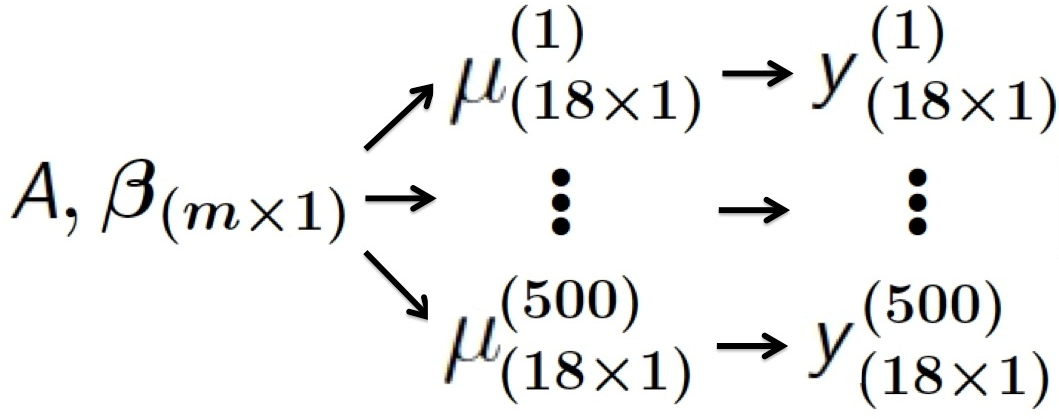
\includegraphics[width=5cm]{process.png}
\caption{Pseudo-data generating process}
\end{center}
\end{figure}

\subsection{Simple Unbiased Estimates of Coverage Probabilities}
Based on the generated pseudo-data sets, let's define an indicator variable, $I_{ij}$, which is 1 if $j$-th player's interval estimate from $i$-th pseudo-data set includes $p_{ij}$ and 0 otherwise. One way to estimate the coverage probability is taking average over these indicator variables. We call it a simple unbiased coverage probability estimate. For example, $\bar{I}_{1}=\sum_{i=1}^{500}I_{i1}/500$ is the estimated coverage probability for the first player.

\subsection{Rao-Blackwellized Unbiased estimates of Coverage Probabilities}
Rao-Blackwellization improves accuracy of an unbiased estimator by taking conditional expectation given a sufficient statistic. Based on this idea, we define $E(I_{ij}\vert z_{ij}, r, \beta$), where $r$ and $\beta$ were given at first (see 5.1) and $z_{ij}$ is a sufficient statistic. This expectation is the same as Pr$(\hat{p}_{ij, low}\le p_{ij} \le\hat{p}_{ij, upp}\vert z_{ij}, r, \beta)$, where ($\hat{p}_{ij, low}$, $\hat{p}_{ij, upp}$) is $j$-th player's interval estimates on the $i$-th data set. We can calculate this probability  because we know the distribution of $p_{ij} \vert z_{ij}, r, \beta$ in (9). Note that conditioning on $z_{ij}$ is equivalent to conditioning on $\mathbf{z}$ as long as $r$ and $\beta$ are known. Then, we can estimate the first player's coverage probability by $\sum_{i=1}^{500}E(I_{i1}\vert z_{i1}, r, \beta)/500$, which is also unbiased but more accurate than the previous simple estimator.

\section[Examples]{Examples}
\subsection[Known Second-level Mean]{31 Hospitals: Known Second-level Mean}
Suppose you live in the New York state (NY) and have been suffering from severe coronary heart disease (hopefully not). If you are supposed to receive the coronary artery bypass graft (CABG) surgery soon, you might want to find the most famous hospital for dealing with such a surgery. On top of that, if you can figure out each hospital's abililty to handle this surgery, it will be useful for your decision in choosing a hospital.
\\

For this purpose, you gathered data of 31 hospitals in NY composed of the number of deaths within a month of CABG surgeries and total number of patients receiving CABG surgeries in each hospital. In addition, while one looks for such information, suppose one knows that the state-level death rate per exposure of this surgery is 0.020. 
\\

The multilevel modeling that assumes a bigger population-level hierarchy will be insightful in this problem. Here, we presume a state-level (NY) hierarchy governing the true death rates of CABG surgery of all the hospitals in NY. This perspective is to view the true death rates of those 31 hospitals as sampled from the state-level population distribution whose mean is 0.020. For reference, a model check can be useful for evaluating the validity of such a view point (Christiansen and Morris, 1996). 
\\

Assuming an additional hierarchy is reasonable, a model-fitting process begins.  Since the true death rate per exposure after CABG surgery might be small and the caseload ($n_{j}$) is much bigger than the number of deaths ($z_{j}$) in each hospital, the Poisson distribution would be our first choice to describe the uncertainty in our data. Next, \code{gbp} will help us fit the Poisson multilevel model with the Gamma conjugate prior distribution on the true death rate $\lambda_{j}$ whose mean is 0.020 ($\lambda_{0}=0.020$) as described in 3.2 . For reference, the number of regression coefficients ($m$) is 0 because we do not need to estimate the prior mean via log-linear regression (see section 3.2).
\begin{CodeChunk}
\begin{CodeInput}
R> p <- gbp(z, n, mean.PriorDist = 0.02, model = "pr")
R> p
\end{CodeInput}
\begin{CodeOutput}
Summary for each unit (sorted by n):

         obs.mean    n prior.mean shrinkage low.intv post.mean upp.intv post.sd
1           0.045   67       0.02     0.834    0.011     0.024    0.042   0.008
2           0.029   68       0.02     0.832    0.010     0.022    0.038   0.007
3           0.024  210       0.02     0.616    0.011     0.021    0.035   0.006
4           0.043  256       0.02     0.568    0.017     0.030    0.046   0.008
5           0.033  269       0.02     0.556    0.015     0.026    0.041   0.007
6           0.044  274       0.02     0.551    0.018     0.031    0.047   0.008
7           0.043  278       0.02     0.548    0.018     0.030    0.047   0.007
8           0.014  295       0.02     0.533    0.008     0.017    0.029   0.005
9           0.029  347       0.02     0.492    0.014     0.024    0.038   0.006
10          0.037  349       0.02     0.491    0.017     0.029    0.043   0.007
11          0.039  358       0.02     0.484    0.018     0.030    0.045   0.007
12          0.018  396       0.02     0.459    0.010     0.019    0.030   0.005
13          0.028  431       0.02     0.438    0.015     0.024    0.037   0.006
14          0.025  441       0.02     0.433    0.013     0.023    0.035   0.005
15          0.027  477       0.02     0.414    0.015     0.024    0.036   0.006
16          0.045  484       0.02     0.410    0.023     0.035    0.050   0.007
17          0.030  494       0.02     0.405    0.016     0.026    0.039   0.006
18          0.022  501       0.02     0.402    0.012     0.021    0.032   0.005
19          0.028  505       0.02     0.400    0.015     0.025    0.036   0.005
20          0.020  540       0.02     0.384    0.012     0.020    0.031   0.005
21          0.028  563       0.02     0.374    0.016     0.025    0.037   0.005
22          0.024  593       0.02     0.362    0.014     0.022    0.033   0.005
23          0.015  602       0.02     0.358    0.010     0.017    0.026   0.004
24          0.024  629       0.02     0.348    0.014     0.023    0.033   0.005
25          0.020  636       0.02     0.346    0.012     0.020    0.030   0.005
26          0.048  729       0.02     0.316    0.027     0.039    0.053   0.007
27          0.031  849       0.02     0.284    0.019     0.028    0.038   0.005
28          0.027  914       0.02     0.269    0.017     0.025    0.035   0.005
29          0.021  940       0.02     0.264    0.014     0.021    0.030   0.004
30          0.029 1193       0.02     0.220    0.020     0.027    0.036   0.004
31          0.020 1340       0.02     0.201    0.014     0.020    0.027   0.003
colMeans    0.029  517       0.02     0.438    0.015     0.025    0.037   0.006
\end{CodeOutput}
\end{CodeChunk}
For reference, we need to type `\code{R> print(p, sort = FALSE)}' instead of `\code{R> p}' in order to list hospitals by the order of data input in the above output. `\code{R> p}' automatically sorts the output by the increasing order of caseload ($n_{j}$). 
\\

The output contains information about sample mean (\code{obs.mean}), caseload (\code{n}), known prior mean ($\lambda_{0}$), shrinkage estimate ($\hat{B}_{j}$), lower interval, posterior mean ($E(\lambda_{j}\vert \textbf{z})$), upper interval, and standard deviation of posterior distribution ($sd(\lambda_{j}\vert \textbf{z})$).
\\

As we can see in (6), the posterior mean, $(1-B_{j})y_{j} + B_{j}\lambda_{0}$, is a linear function of shrinkage, $B_{j}\equiv r / (r + n_{j})$, locating between the sample mean and prior mean ($\lambda_{0}=0.02$). It makes sense because $r$ can be interpreted as the amount of prior information and $n_{j}$ as the amount of observed information. If the second level has more information than the first level, then the sample mean shrinks towards the prior mean more than 50\%. This point is clear in the above output because, as caseload increases, shrinkage decreases, depending less on the prior distribution.
\\

A function ``\code{summary}'' shows selective information on hospitals and more detailed estimation result as below. To be specific, it displays some hospitals (not all as above) with minimum, median, and maximum caseloads ($n_{j}$). On top of that, more specific estimation results, such as the estimation result of $\alpha\equiv\log(1/r)$, follow. Note that when we do not know the prior mean in advance unlike this hospital problem, \code{gbp} fits a linear regression for the Normal model, a log-linear regression for the Poisson model, or a logistic regression for the Binomial model and a summary of regression fit will appear.
\begin{CodeChunk}
\begin{CodeInput}
R> summary(p)
\end{CodeInput}
\begin{CodeOutput}
Main summary:

                  obs.mean    n prior.mean shrinkage low.intv post.mean
Unit w/ min(n)       0.045   67       0.02     0.834    0.011     0.024
Unit w/ median(n)    0.045  484       0.02     0.410    0.023     0.035
Unit w/ max(n)       0.020 1340       0.02     0.201    0.014     0.020
Overall Mean         0.029  517       0.02     0.438    0.015     0.025

                  upp.intv post.sd
                     0.042   0.008
                     0.050   0.007
                     0.027   0.003
                     0.037   0.006

Second-level Variance Component Estimation Summary:
alpha = log(A) for Gaussian and log(1/r) for Binomial and Poisson data:

  post.mode.alpha post.sd.alpha
1          -5.818         0.411
\end{CodeOutput}
\end{CodeChunk}
Since estimated $\alpha$ is -5.818, we can easily calculate $\hat{r}=\textrm{exp}(5.818)=336$, which is a good indicator of how valuable and informative the hypothetical second-level hierarchy is. Note that $r$ can be interpreted as the amount of prior information, although we do not know its true value. So, \code{gbp} asked data how much credit they wanted to give to this hypothetical second-level hierarchy. $\hat{r}$ = 336 is the answer from the data. It means that observed sample means of hospitals whose caseloads are less than 336 will shrink toward the prior mean (0.020) more than 50\%. 
\\

For example, the shrinkage estimate of the first hospital ($\hat{B}_{1}= 0.834$) was calculated by 336 / (336 + 67), where 67 is its caseload ($n_{1}$), and its posterior mean is $(1-0.834)*0.045 + 0.834 * 0.020=0.024$. As for this hospital, using more information from the prior distribution is an appropriate choice because its observed amount of information (67) is far less than the amount of state-level information (336).
\\

We also need a graphical summary that can give us valuable insight buried in pile of numbers and a function `\code{plot}' is exactly for this purpose.
\begin{CodeChunk}
\begin{CodeInput}
R> plot(p)
\end{CodeInput}
\end{CodeChunk}
\begin{figure}[h]
\begin{center}
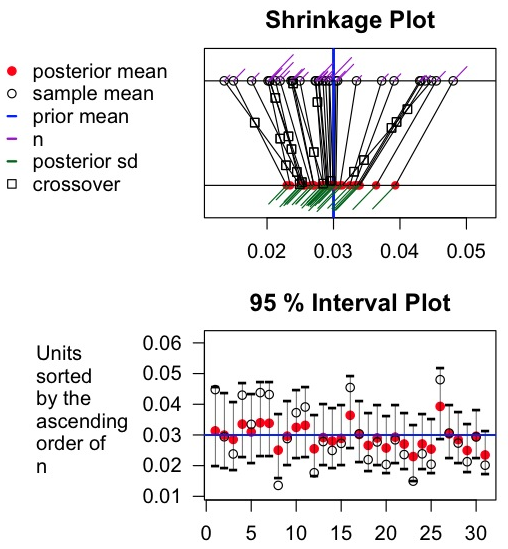
\includegraphics[scale=0.25]{hospital1.png}
\end{center}
\end{figure}

The regression towards the mean (RTTM) is obvious in the left-side graph; the observed sample means, empty dots on the upper line, are shrinking towards the known second-level mean (a blue vertical line at 0.02) to the different extents. Note that some hospitals' ranks have changed by shrinking much harder towards 0.02 than others. For example, the empty square symbol at the crossing point of the two left-most lines (8th and 23rd hospitals on the list above) indicates that seemingly safest hospital among 31 hospitals in terms of the observed sample mean was not actually safer than the second safest hospital. Without this hierarchical modeling, we might have made a wrong decision in choosing a hospital.
\\

Intuitively, the result of multilevel modeling makes more sense than that of naive sample mean. For example, suppose there are two hospitals, whose sample means ($z_{j} / n_{j}$) are 0 and 0.001 and caseloads ($n_{j}$) are 1 and 1000 each. Do you believe that the former hospital, whose observed death rate is 0, is better than the latter and are you going to choose the former hospital? Borrowing information from state-level hierarchy seems reasonable for the former hospital because it is hard to judge its true death rate per exposure with just one caseload. Though somewhat extreme, this is what happened to the two left-most hostpitals in the first plot and this is why hierarchical modeling is a reasonable choice for this data set.
\\

The estimated 95\% intervals are displayed on the right-side plot. We can clearly see that all the posterior means (red dots) are between sample mean (empty dots) and second-level mean (a blue horizontal line). For reference, if we want to draw this plot by the order of data input, \code{plot(p, sort = FALSE)} is a right adjustment. Overall, as the caseload increases towards the right and as the posterior mean gets closer to 0, the length of interval gets shorter, which the formula of posterior variance in (6) implies. 
\\

This interval plot can give us one more valuable insight, which we could not have noticed. Let's look at the 8th and the 31st hospitals on the graph (or on the outcome for numeric reference). The point estimate of the true death rate per exposure of the 31st hospital is higher than the one of the 8th. But, the upper bound of interval estimate of this 31st hospital is lower than that of the 8th. This interval plot makes the 31st hospital emerge as one of your candidates. (Could you regard this 31st hospital as a possible candidate before you observe this plot?)
\\

Also it reveals that the 23rd hospital, whose estimated true rate was the smallest, has also the smallest upper bound. If you are a risk-avoider, this hospital will attract you most strongly. And if you already chose this 23rd hospital compared to the 8th from the shrinkage plot, your decision might become stronger at this point, excluding the 8th hospital with more certainty. 
\\

Then, how reliable are these intervals? Does our procedure to generate interval estimates have good repeated sampling property? The following method check will answer this question. The \code{coverage} function below generates 10,000 pseudo-data sets regarding the estimated $r~(=336.37)$ as a given true value. For reference, we can try any other value of $r$, for example $r=200$, by replacing below code with `\code{R> pcv <- coverage(p, A.or.r = 200, mean.PriorDist = 0.02, nsim = 10000)}.
\\

Also, \code{gbp} can give us interval estimates with different confidence level, for example 90\%,  and the appropriate code adjustment is \code{R> p <- gbp(z, n, Alpha = 0.9, mean.PriorDist = 0.02, model = "pr")}.  Then, the function \code{coverage} will evaluate whether interval estimates achieve 90\% confidence level.
\\

\begin{CodeChunk}
\begin{CodeInput}
R> pcv <- coverage(p, nsim = 10000)
\end{CodeInput}
\end{CodeChunk}
\begin{figure}[h]
\begin{center}
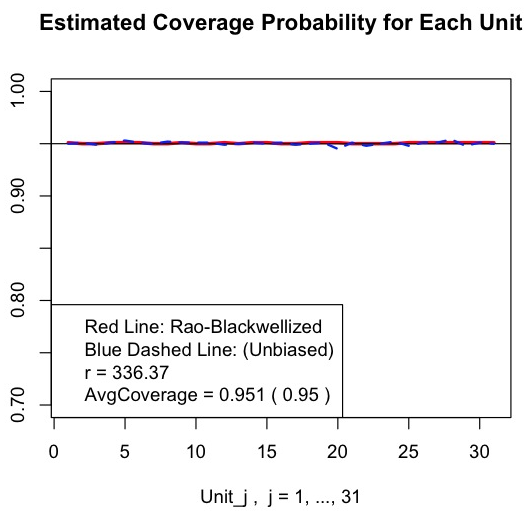
\includegraphics[width = 5.5cm]{hospital2.png}
\end{center}
\end{figure}

It estimated coverage probabilities by simple unbiased estimates (a blue dashed line) and Rao-Blackwellized unbiased estimates (a red line). Both lines are indistingishable from the horizontal line at 0.95 and the estimated overall average coverage rate is 0.950 from the Rao-Blackwellized estimate and 0.951 from the simple unbiased estimate. Considering this result, we finally conclude that the interval estimates from the suggested multilevel modeling on this particular data set has nice repeated sampling property.
\\

%These numbers are encouraging, but achieving at least 95\% coverage at %one specific true value does not mean that our model has good repeated %sampling property. We need to check whether coverage probabilities are %at least 0.95 when the true parameter value ($r$) varies.

%\begin{CodeChunk}
%\begin{CodeInput}
%R> shr <- seq(0.01, 0.99, length.out = 20)
%R> r.trial <- mean(n) * shr / (1 - shr)
%R> cov.save <- sapply (1 : length(r.trial), function(i){
%R>               coverage(p, A.or.r = r.trial[i], mean.PriorDist = 0.02, 
%R>                        nsim = 500)$average.coverageRB
%R>             })
%\end{CodeInput}
%\end{CodeChunk}
%\begin{figure}[h]
%\begin{center}
%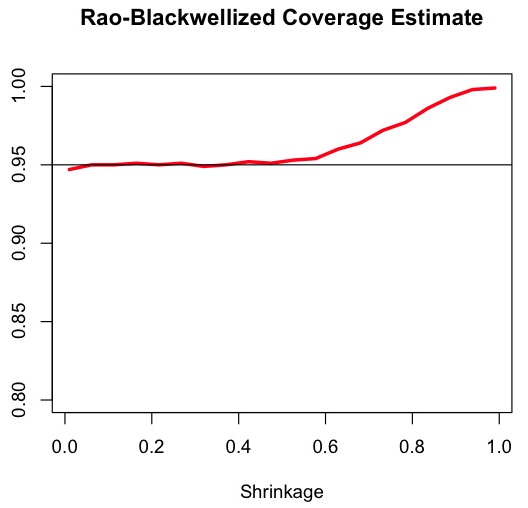
\includegraphics[width = 5.5cm]{hospital3.png}
%\end{center}
%\end{figure}

%We plotted \code{cov.save} on \code{shr}, connecting dots (coverage %probabilities). This plot shows that the estimated shrinkages are at least %0.947 (under 95\% only at one shrinkage value, 0.01) on the tried range %of true shrinkage values, slightly deviating from the definition of 95\% %confidence interval. Note that our model is approximating the true %distribution of shrinkage by ADM (see 4.2). 

%The reason we tried true shrinkage values between 0.01 and 0.99 is that no shriankge ($\equiv r / (r + n_{j})=0)$, corresponding to $r=0$, makes the scale of the distribution go to $\infty$ (see (5)), and full shrinkage ($B_{j}=1$) makes $r$ goes to $\infty$, not appropriate for an argument.

Morris and Christiansen (1995) also looked into a similar ranking problem in hierarchical modeling, taking shrinkage into account.
\\

\subsection[Unknown Second-level Mean and No Covariate]{8 Schools: Unknown Second-level Mean and No Covariate}
\begin{CodeChunk}
\begin{CodeInput}
R> g <- gbp(y, se, model = "gr")
R> g
\end{CodeInput}
\begin{CodeOutput}
Summary for each unit (sorted by n):

         obs.mean   se prior.mean shrinkage low.intv post.mean upp.intv post.sd
5           -1.00  9.0      8.168     0.408  -13.297     2.737   16.692   7.634
2            8.00 10.0      8.168     0.459   -7.255     8.077   23.361   7.810
7           18.00 10.0      8.168     0.459   -1.289    13.484   30.821   8.176
4            7.00 11.0      8.168     0.507   -8.780     7.592   23.602   8.257
6            1.00 11.0      8.168     0.507  -13.027     4.633   20.131   8.441
1           28.00 15.0      8.168     0.657   -2.315    14.979   38.763  10.560
3           -3.00 16.0      8.168     0.685  -17.130     4.650   22.477  10.096
8           12.00 18.0      8.168     0.734  -10.208     9.189   29.939  10.227
colMeans     8.75 12.5      8.168     0.552   -9.163     8.168   25.723   8.900
\end{CodeOutput}
\end{CodeChunk}

\begin{CodeChunk}
\begin{CodeInput}
R> summary(g)
\end{CodeInput}
\begin{CodeOutput}
Main summary:

                    obs.mean   se prior.mean shrinkage low.intv post.mean
Unit w/ min(se)        -1.00  9.0      8.168     0.408  -13.297     2.737
Unit w/ median(se)1     1.00 11.0      8.168     0.507  -13.027     4.633
Unit w/ median(se)2     7.00 11.0      8.168     0.507   -8.780     7.592
Unit w/ max(se)        12.00 18.0      8.168     0.734  -10.208     9.189
Overall Mean            8.75 12.5      8.168     0.552   -9.163     8.168

                     upp.intv post.sd
                       16.692   7.634
                       20.131   8.441
                       23.602   8.257
                       29.939  10.227
                       25.723   8.900

Second-level Variance Component Estimation Summary:
alpha = log(A) for Gaussian and log(1/r) for Binomial and Poisson data:

  post.mode.alpha post.sd.alpha
1           4.768         1.139


Regression Summary:

      estimate   se z.val p.val
beta0    8.168 5.73 1.425 0.154
\end{CodeOutput}
\end{CodeChunk}

%\begin{figure}[h]
%\begin{center}
%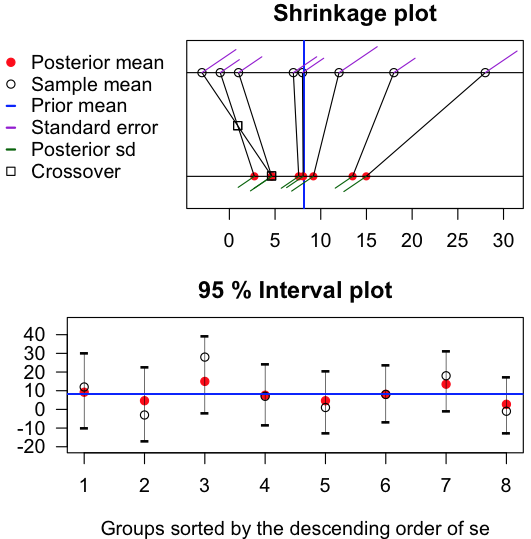
\includegraphics[scale=0.3]{school1.png}
%\caption{Shrinkage and interval plots of 8 schools}
%\end{center}
%\end{figure}

%\begin{CodeChunk}
%\begin{CodeInput}
%R> gcv <- coverage(g, nsim = 10000)
%\end{CodeInput}
%\end{CodeChunk}
%\begin{figure}[h]
%\begin{center}
%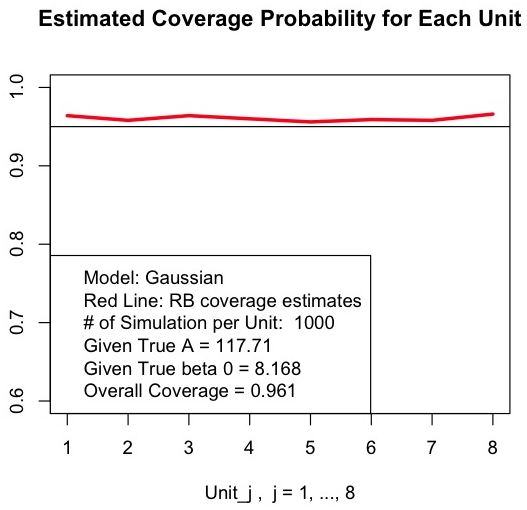
\includegraphics[width = 5.5cm]{school2.png}
%\end{center}
%\end{figure}

%\begin{CodeChunk}
%\begin{CodeInput}
%R> shr <- seq(0.01, 0.99, length.out = 20)
%R> A.trial <- mean(n) * (1 - shr) / shr
%R> cov.save <- sapply (1 : length(A.trial), function(i){
%R>               coverage(g, A.or.r = A.trial[i], reg.coef = 8.168, 
%R>                        nsim = 500)$average.coverageRB
%R>             })
%\end{CodeInput}
%\end{CodeChunk}
%\begin{figure}[h]
%\begin{center}
%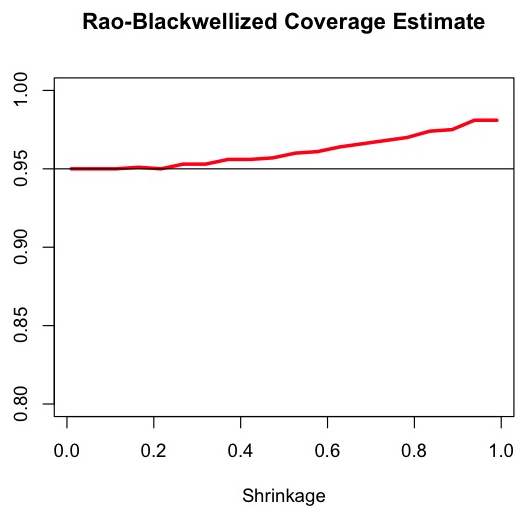
\includegraphics[width = 5.5cm]{school3.png}
%\end{center}
%\end{figure}


\subsection[Unknown Second-level Mean and One Covariate]{18 Baseball Players: Unknown Prior Mean and One Covariate}
In this example, suppose you read the New York Times published on 26 April 1970. One article in this magazine covered 18 baseball players' batting averages through their first official 45 at-bats of the 1970 season. And then, you became interested in their batting averages over the remaining season. How could you predict? For reference, the data set  \code{baseball} has each player's batting average over the remaining season. 
\\

First of all, the independent Binomial distribution given a true batting average of each player (see (7)) seems an appropriate probability distribution describing the uncertainty in this data set. And we know that the sample mean (MLE) under this distribution is an uniformly minimum variance unbiased estimator (UMVUE) with nice asymptotic properties. It is also the simplest way to estimate their true batting averages. But can we say this is the best way to predict their batting averages?
\\

Efron and Morris (1975) said ``no,'' and suggested James-Stein estimator, making each players' sample mean shrink towards an estimated mean of the second-level prior distribution. They showed that this estimator was more than three times efficient than the sample mean under squared error loss. On top of that, a few years later Morris (1983) introduced interval estimates that could successfully catch the batting averages over the remaining season, which MLE and its interval estimate could not.
\\

Our hierarchical modeling is a sequel to these researches, which can add one more unique value. Suppose you strongly believe that the outfielder's batting averages are different from other positions' ones, not giving a credit to the assumption that all players' batting averages shrink towards the same mean. Instead, you want to assume two different second-level hierarchies for outfielders and for other positions, within each of which sharing information and regressing toward the mean (RTTM) occur. This perspective considers true batting averages of outfielders as sampled from the one and those of other positions from the other. Our multilevel modeling provides a way to incorporate such information (covariate) seamlessly into the second-level hierarchy.
\begin{CodeChunk}
\begin{CodeInput}
R> b <- gbp(z, n, x, model = "br")
R> b
\end{CodeInput}
\begin{CodeOutput}
Summary for each unit (sorted by n):

         obs.mean  n   X1 prior.mean shrinkage low.intv post.mean upp.intv post.sd
1           0.400 45 1.00      0.310     0.715    0.248     0.335    0.429   0.046
2           0.378 45 1.00      0.310     0.715    0.244     0.329    0.420   0.045
3           0.356 45 1.00      0.310     0.715    0.240     0.323    0.411   0.044
4           0.333 45 1.00      0.310     0.715    0.236     0.316    0.403   0.043
5           0.311 45 1.00      0.310     0.715    0.230     0.310    0.396   0.042
6           0.311 45 0.00      0.233     0.715    0.179     0.256    0.341   0.041
7           0.289 45 0.00      0.233     0.715    0.175     0.249    0.331   0.040
8           0.267 45 0.00      0.233     0.715    0.171     0.243    0.323   0.039
9           0.244 45 0.00      0.233     0.715    0.166     0.237    0.315   0.038
10          0.244 45 1.00      0.310     0.715    0.210     0.291    0.379   0.043
11          0.222 45 0.00      0.233     0.715    0.161     0.230    0.308   0.038
12          0.222 45 0.00      0.233     0.715    0.161     0.230    0.308   0.038
13          0.222 45 0.00      0.233     0.715    0.161     0.230    0.308   0.038
14          0.222 45 1.00      0.310     0.715    0.202     0.285    0.375   0.044
15          0.222 45 1.00      0.310     0.715    0.202     0.285    0.375   0.044
16          0.200 45 0.00      0.233     0.715    0.155     0.224    0.302   0.038
17          0.178 45 0.00      0.233     0.715    0.148     0.218    0.297   0.038
18          0.156 45 0.00      0.233     0.715    0.140     0.211    0.292   0.039
colMeans    0.265 45 0.44      0.267     0.715    0.191     0.267    0.351   0.041
\end{CodeOutput}
\end{CodeChunk}
Our model reflects on the additional information, \emph{i.e.}, indicator covariate (1 for outfielder and 0 for other positions), estimating two different prior means, 0.310 and 0.233. Also note that shrinkage estimates are the same for all players. It makes sense because shrinkage ($B_{j}\equiv r / (r+n_{j})$) is determined by the relative amount of information between the first-level and the second-level hierarchies. The fact that all players have the same amount of observed information ($n_{j}=45$) and $\hat{r}=\textrm{exp}(4.727)=113$ from below summary tell why the estimated shrinkage is 0.715 (=113 / (113 + 45)).
\\

For reference, we can run the Normal hierarchical model using $y_{j}=z_{j} / n_{j}$ and $V_{j}=\bar{y}(1-\bar{y})/n$, where $\bar{y}=\sum_{j} z_{j} / \sum_{j} n_{j}$, $j=1,\ldots, 18$. For comparison, we calculated squared error losses, $\sum_{j=1}^{18}(p_{j, remaining}-\hat{p}_{j})^{2}$, using the estimates from the Binomial and Normal multilevel models and also using the sample mean (MLE). These values were 0.042, 0.043, and 0.086 each. Note that estimates from the Normal and Binomial models are twice better than MLE in terms of squared error loss. 
\\

One more thing to note is that the posterior standard deviation tends to be bigger among outfielders than among others. Let's see its formula in (9). We can notice that the estimated posterior mean is one factor that determines posterior variance because every player has the same at-bats ($n_{j}$) and $r$. As the posterior mean gets closer to 0.5, the posterior variance gets bigger and has the biggest value when the posterior mean is 0.5. Intuitively, it makes sense. If a true batting average is 0.1, we can easily expect less hits. But if it is 0.5, we are less certain whether an at-bat would be more likely a hit or not, like a coin tossing. Our model is automatically reflecting on such uncertainty.
\begin{CodeChunk}
\begin{CodeInput}
R> summary(b)
\end{CodeInput}
\begin{CodeOutput}
Main summary:

                          obs.mean  n   X1 prior.mean shrinkage low.intv
Unit w/ min(obs.mean)        0.156 45 0.00      0.233     0.715    0.140
Unit w/ median(obs.mean)1    0.244 45 0.00      0.233     0.715    0.166
Unit w/ median(obs.mean)2    0.244 45 1.00      0.310     0.715    0.210
Unit w/ max(obs.mean)        0.400 45 1.00      0.310     0.715    0.248
Overall Mean                 0.265 45 0.44      0.267     0.715    0.191

                         post.mean upp.intv post.sd
                             0.211    0.292   0.039
                             0.237    0.315   0.038
                             0.291    0.379   0.043
                             0.335    0.429   0.046
                             0.267    0.351   0.041

Second-level Variance Component Estimation Summary:
alpha = log(A) for Gaussian and log(1/r) for Binomial and Poisson data:

  post.mode.alpha post.sd.alpha
1          -4.727         0.957


Regression Summary:

      estimate    se  z.val p.val
beta0   -1.194 0.131 -9.129 0.000
beta1    0.389 0.187  2.074 0.038
\end{CodeOutput}
\end{CodeChunk}

This summary also includes the result of logistic regression fit because we did not know prior means in advance so that we had to estimate them via this logistic regression model. Let's look at the p-value of the indicator covariate (\code{beta1}). It shows that the two different prior distributions distinguishing outfielders from other positions were significantly different, supporting our assumption. The positive sign of $\hat{\beta}_{1}$ reflects on the first five players, outfielders, whose observed batting averages were higher than others.
\\
\begin{CodeChunk}
\begin{CodeInput}
R> plot(b)
\end{CodeInput}
\end{CodeChunk}
\begin{figure}[h]
\begin{center}
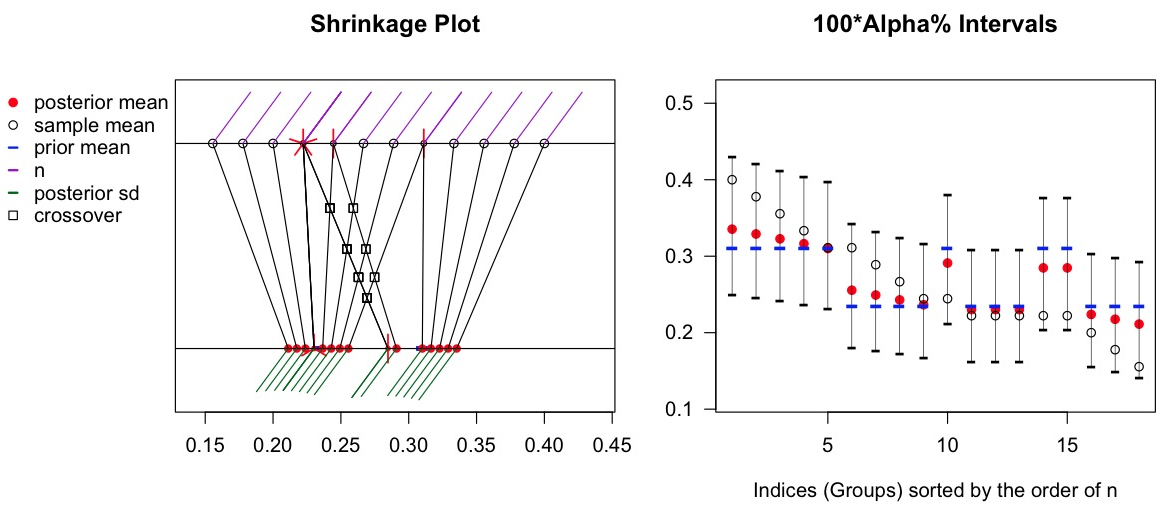
\includegraphics[scale=0.3]{baseball1.png}
\end{center}
\end{figure}

Let's see shrinkage and 95\% interval plots for more intuition. It is obvious that sample means (empty dots) on the upper line shrink towards two different means, 0.310 and 0.233. For reference, the red line symbols on dots are for when two or more points have the same mean and are plotted over each other. For example, five players (from the 11th player to the 15th) have the same sample mean (0.222) and at this point on the upper line, there are short red lines toward five directions. This symbol also means that the seemingly two lines crossing over others were actually three lines for those who were outfielders (10th, 14th, and 15th hitters) with observed batting averages far lower than the top five hitters.
\\

Note that the observed sample mean among outfielders is 0.308 and that among other positions is 0.231. But why are the estimated two prior means from this Binomial model 0.310 and 0.233 each? This can be attributed to the logistic regression which estimates prior mean by a non-linear logit function of $x'\beta$, causing a small bias (see 3.3). The Normal model can avoid this small bias because it uses a linear regression to estimate these prior means.
\\

The 95\% interval plot shows us range of true batting average for each player, which clarifies the regression toward the mean (RTTM) within two groups. Let's see the 10th, 14th, and 15th players on the graph for example. They are outfielders but their batting averages (sample mean) are far worse than the first five outfielders. RTTM means that it can happen by their bad luck though in the long run their batting averages will come back to their expected ones as outfielders (blue horizontal line). The fact that their sample means are located at the lower part of their 95\% intervals supports this argument. So, their posterior means (red dots) can also be interpreted as their RTTM. 
\\

One more thing to emphasize is that observed sample means are all within the interval estimates. And these interval estimates also catched the batting averages over the ramaining season successfully, although the result was left out. Then, how much can we trust these interval estimates? The following method check will answer it. 

\begin{CodeChunk}
\begin{CodeInput}
R> bcv <- coverage(b, nsim = 10000)
\end{CodeInput}
\end{CodeChunk}
\begin{figure}[h]
\begin{center}
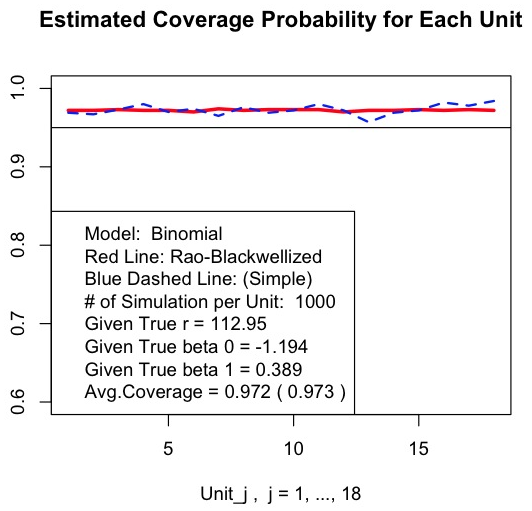
\includegraphics[width = 5.5cm]{baseball2.png}
\end{center}
\end{figure}

The meaning of putting the \code{gbp} object, \code{b}, without any additional argument in the above \code{coverage} function is to make this function regard the estimated values, such as $\hat{r}$ (=112.95) and $\hat{\beta}~(=(-1.194, ~0.389)^{T})$, as true values for generating pseudo-data sets. 
\\

Finally, the estimated average coverage probability is 0.973 based on the Rao-Blackwellization, conservatively satisfying the definition of the 95\% confidence interval. 
\\

%However, achieving at least 95\% coverage at specific true values of $r$ and $\beta$ does not mean that our model has good repeated sampling property. So, as we did in previous examples, we will see whether coverage probabilities are at least 0.95 when the true shrinkage value ($B(r)$) varies, fixing $\beta$ at estimated values. Note that, if we want to check a coverage probability under the different parameter values, $r$ and $\beta$, for example 150 for $r$ and $(-1, 0.5)^{T}$ for $\beta$, the appropriate code is \code{R> coverage(b, A.or.r = 150, reg.coef = c(-1, 0.5), covariates = x, nsim = 10000)}. 

%\begin{CodeChunk}
%\begin{CodeInput}
%R> shr <- seq(0.01, 0.99, length.out = 20)
%R> r.trial <- mean(n) * shr / (1 - shr)
%R> cov.save <- sapply (1 : length(r.trial), function(i){
%R>               coverage(b, A.or.r = r.trial[i], reg.coef = c(-1.194, 0.389), 
%R>                        covariates = x, nsim = 500)$average.coverageRB
%R>             })
%\end{CodeInput}
%\end{CodeChunk}
%\begin{figure}[h]
%\begin{center}
%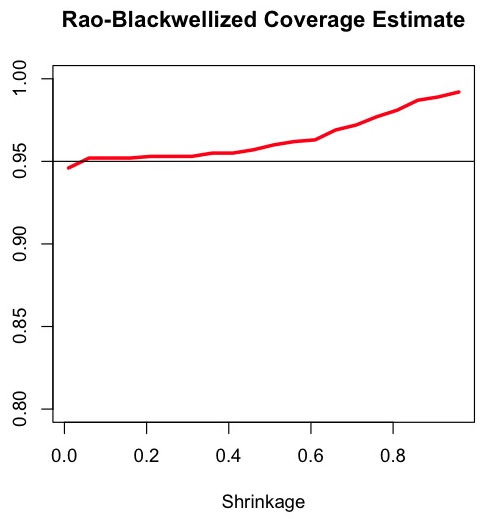
\includegraphics[width = 5.5cm]{baseball4.png}
%\end{center}
%\end{figure}

%We drew \code{cov.save} on \code{shr}, conneting dots. It shows that the estimated shrinkages are at least 0.946 on the tried range of true shrinkage values, slightly deviating from the definition of 95\% confidence interval. Note that even this result does not guarantee good repeated sampling property because $\beta$ was fixed. But, this result can definitely be an encouraging sign for our model's good repeated sampling property. 

%The reason we tried true shrinkage values between 0.01 and 0.99 is that no shriankge ($\equiv r / (r + n_{j}))$, corresponding to $r=0$, makes parameters of the second-level distribution 0 (see (8)), and full shrinkage corresponds to $r=\infty$ that we cannot designate as an argument of \code{coverage} function.

\section[Discussion]{Discussion}
Bayes vs Freq, post.mean vs estimate, post.sd vs estimated standard error.
\section[acknowledgments]{Acknowledgments}

\section[Reference]{Reference}
1. Christiansen, C. and Morris, C. (1996). ``Fitting and Checking a Two-Level Poisson Model: Modeling Patient Mortality Rates in Heart Transplant Patients,'' in \emph{Bayesian Biostatistics}, eds. D. Berry and D. Stangl, New York: Marcel Dekker, pp. 467-561.
\\

2. Efron, B. and Morris, C. (1975). ``Data Analysis Using Stein's Estimator and its Generalizations.'' \emph{Journal of the American Statistical Association}. \textbf{70}. 311-319.
\\

3. Kass, R. and Steffey, D. (1989). ``Approximate Bayesian Inference in Conditionally Independent Hierarchical Models (Parametric
Empirical Bayes Models).'' \emph{Journal of the American Statistical Association}. \textbf{84}. 717-726.
\\

4. Morris, C. (1983). ``Parametric Empirical Bayes Inference: Theory and Applications.'' \emph{Journal of the American Statistical Association}. \textbf{78}. 47-55.
\\

5. Morris, C. and Christiansen, C. (1995). ``Hierarchical Models for Ranking and for Identifying Extremes, With Application,'' in \emph{Bayesian Statistics 5}, eds. J. Bernardo, J. Berger, A. Dawid, and A. Smith, New York: Oxford University Press, pp. 277-296.
\\

6. Morris, C. and Tang, R. (2011). ``Estimating Random Effects via Adjustment for Density Maximization.'' \emph{Statistical Science}. \textbf{26}. 271-287.
\\

7. Morris, C. and Lysy, M. (2012). ``Shrinkage Estimation in Multilevel Normal Models.'' \emph{Statistical Science}. \textbf{27}. 115-134.
\\

8. Rubin, D. B. (1981). ``Estimation in parallel randomized
  experiments.'' \emph{Journal of Educational Statistics}. \textbf{6}. 377-401.
\\


\end{document}
